\newpage
\section{Miniboxing Encoding}
\label{mbox:sec-miniboxing}

\topic{Constraints on the bytecode size currently prevent us from extending the use of specialization in the standard library,} namely, to tuples of three elements, to the collections hierarchy and to |Function| traits, which are used in Scala's object oriented representation of functions. Therefore we propose the miniboxing encoding and transformation as a solution to reduce bytecode size and allow library specialization. Along with the encoding, we present a transformation based on the principles of specialization, but using the miniboxed encoding (\S\ref{mbox:sec-mb-traf}) instead of primitive value types.

The miniboxing technique relies on a simple insight: grouping different value types reduces the number of variants necessary in the heterogeneous translation. To this end, we need to group the value types in the language into disjoint sets and for each set designate a value type, also called a storage type, which can encode any type in that set. Notice that this definition is not limited to primitive value types, but can also be used for C-like structs.

Four conditions need to be satisfied for the miniboxing transformation to work:
\begin{itemize}
  \item All of the value types in the language can be encoded into one or more storage types;
  \item The overhead of transforming between any value type and its storage type must be limited, ideally a no-op;
  \item The operations available for generic types in the language (inherited from the top of the hierarchy, such as |toString|, |hashCode| and |equals|) must be fixed;
  \item All the value types need to have boxed representations, to enable compatibility between the miniboxed and homogeneous translations (\S\ref{mbox:subsec-spec-compatibility}). If the bytecode's common representation is tagged union, the requirement changes to having tagged union representations.
\end{itemize}

In this case, the heterogeneous translation only needs to generate variants for the storage types and references. References are a special storage type, since all value types are also considered to be part of the reference group. During the translation, whenever a type is not known to be miniboxed to one of the storage types, it is automatically assumed to be attached to the references group. This allows the opportunistic (\S\ref{mbox:subsec-spec-rewiring}) and compatible (\S\ref{mbox:subsec-spec-compatibility}) rewiring of the tree: indeed since any value type has a boxed representation, it is always correct (but not optimal) to store it as a boxed reference. In the extreme case where all value types are their own storage types, we are back to specialization.

The next subsection will present miniboxing in Scala.

\begin{figure}[t!]
    \centering
    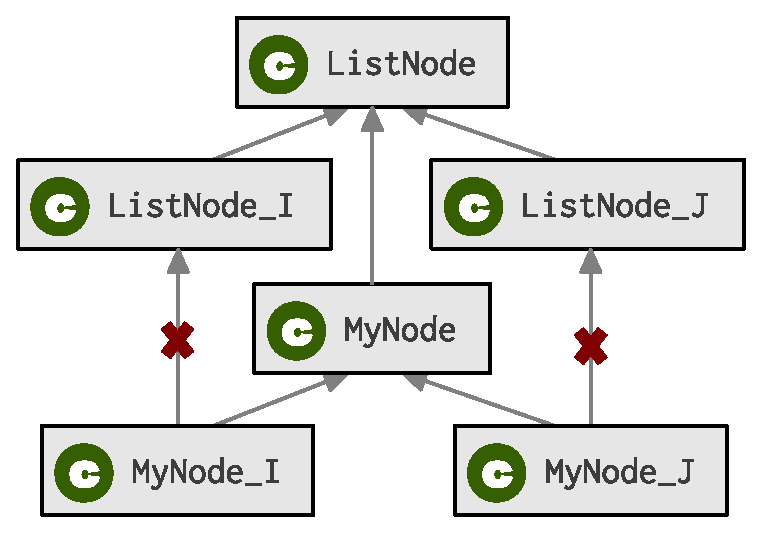
\includegraphics[width=0.50\textwidth]{diags/spec-multi.eps}

    \caption{An example of specialized class inheritance made impossible by the current translation scheme.}
    \label{mbox:fig-spec-multi}

\end{figure}

\subsection{Miniboxing in Scala}

In order to apply the miniboxing encoding to Scala, we decided to use the long integer (|Long|) as the storage type of all other primitive value types. Other sets of storage types could also be implemented to improve specific scenarios, such as running on 32-bit architectures (32-bit |Int| and 64-bit |Long|) or using floating-point numerics extensively\footnote{The floating point to integer bit-preserving transformations, which are implemented as intrinsics, do incur a measurable overhead.} (64-bit |Double| and 64-bit |Long|). Still, for the rest of the description, we will use the long integer as the only storage type, in order to be consistent with the current implementation of the miniboxing plugin.

\topic{The transformation primitives from value types to} |Long| and back are implemented in the HotSpot Java Virtual Machine and have direct translations to bytecode$^\text{4}$ and to processor instructions \cite{intel-ia-32-instruction-reference}. Nevertheless, two concerns need our attention when using miniboxing: %% TODO: Ugly hardcoded footnote
\begin{itemize}
\item Packing and unpacking cost;
\item Memory footprint of the miniboxed encoding.
\end{itemize}

\topic{\textbf{Packing and unpacking cost.} Boxing and unboxing accesses the heap memory. The main goal of miniboxing is to eliminate this overhead,} but, in doing so, conversions to and from long integers must not slow down program execution significantly compared to monomorphic code. Our benchmarks show that indeed the overhead is negligible (\S{}\ref{mbox:sec-evaluation}).

\topic{\textbf{Memory footprint.} The miniboxed encoding has a memory footprint between that of monomorphic and generic code.} Considering byte as the type argument, the memory footprint of the miniboxed encoding is 8 times larger than the one for monomorphic code, which would store the byte directly. This factor is reduced by specializing bulk storage (arrays) and considering the paddings introduced by the virtual machine. On the other hand, when compared to boxing on 64 bit processors, the factor is exactly 1, as both a pointer and a long integer have 8 bytes. And this does not take into account the heap space occupied by the boxed values themselves. Therefore, all things considered, miniboxing has a memory footprint larger than the monomorphic and heterogeneous translations, but smaller than homogeneous translations based on boxing.

% The next section will present the miniboxing translation.